\documentclass[tikz,border=6pt]{standalone}
\usepackage{tikz}
\usetikzlibrary{arrows.meta,positioning}
\definecolor{nebula}{HTML}{6366F1}
\definecolor{spark}{HTML}{14B8A6}
\definecolor{ink}{HTML}{334155}
\begin{document}
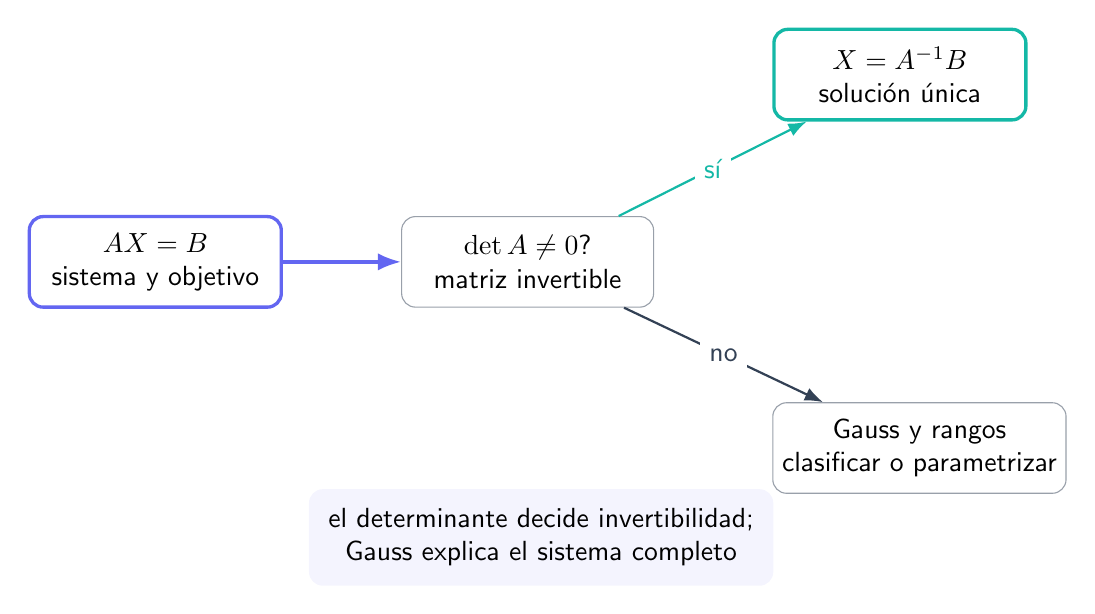
\begin{tikzpicture}[font=\sffamily,>=Latex,node distance=1.5cm,box/.style={draw=ink!50,rounded corners=5pt,minimum width=3.2cm,minimum height=1.15cm,align=center,fill=white}]
  \node[box,draw=nebula,very thick] (system) {$AX=B$\\sistema y objetivo};
  \node[box,right=of system] (det) {$\det A\ne0$?\\matriz invertible};
  \node[box,above right=1.2cm and 1.5cm of det,draw=spark,very thick] (inverse) {$X=A^{-1}B$\\soluci\'on \'unica};
  \node[box,below right=1.2cm and 1.5cm of det] (gauss) {Gauss y rangos\\clasificar o parametrizar};
  \draw[->,very thick,nebula] (system)--(det);
  \draw[->,thick,spark] (det)--(inverse) node[midway,fill=white] {s\'i};
  \draw[->,thick,ink] (det)--(gauss) node[midway,fill=white] {no};
  \node[align=center,fill=nebula!7,rounded corners=5pt,inner sep=7pt] at (4.9,-3.5) {el determinante decide invertibilidad;\\Gauss explica el sistema completo};
\end{tikzpicture}
\end{document}
